\documentclass[tikz,border=10pt]{standalone}
\usepackage{tikz}
\usetikzlibrary{arrows.meta,positioning,calc,decorations.markings}

\begin{document}
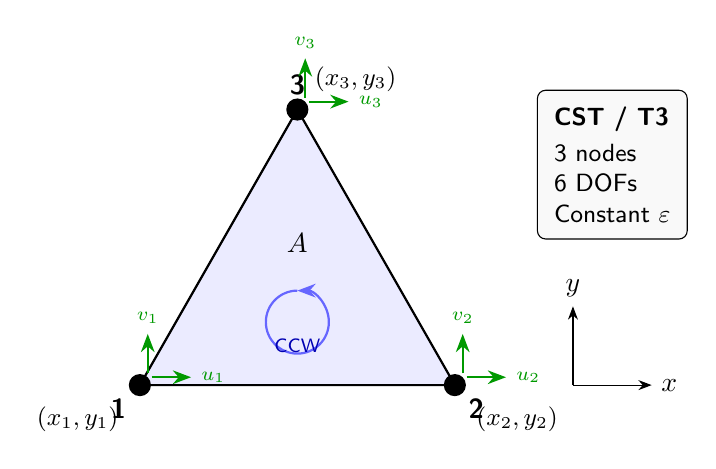
\begin{tikzpicture}[
    node font=\sffamily,
    >=Stealth,
    node dot/.style={circle, fill=black, inner sep=0pt, minimum size=8pt},
    node hollow/.style={circle, draw=black, fill=white, inner sep=0pt, minimum size=8pt, line width=1.2pt},
    dof arrow/.style={->, thick, color=green!60!black},
    dim line/.style={<->, thin, gray},
]

% Triangle fill
\fill[blue!8] (0,0) -- (4,0) -- (2,3.5) -- cycle;

% Triangle edges
\draw[thick] (0,0) -- (4,0) -- (2,3.5) -- cycle;

% Nodes
\node[node dot] (n1) at (0,0) {};
\node[node dot] (n2) at (4,0) {};
\node[node dot] (n3) at (2,3.5) {};

% Node labels
\node[below left=2pt] at (n1) {\textbf{1}};
\node[below right=2pt] at (n2) {\textbf{2}};
\node[above=2pt] at (n3) {\textbf{3}};

% Coordinate labels
\node[below left=6pt, font=\small\itshape] at (n1) {$(x_1, y_1)$};
\node[below right=6pt, font=\small\itshape] at (n2) {$(x_2, y_2)$};
\node[above right=4pt, font=\small\itshape] at (n3) {$(x_3, y_3)$};

% DOF arrows at each node
% Node 1
\draw[dof arrow] (0.15,0.1) -- ++(0.5,0) node[right, font=\scriptsize] {$u_1$};
\draw[dof arrow] (0.1,0.15) -- ++(0,0.5) node[above, font=\scriptsize] {$v_1$};

% Node 2
\draw[dof arrow] (4.15,0.1) -- ++(0.5,0) node[right, font=\scriptsize] {$u_2$};
\draw[dof arrow] (4.1,0.15) -- ++(0,0.5) node[above, font=\scriptsize] {$v_2$};

% Node 3
\draw[dof arrow] (2.15,3.6) -- ++(0.5,0) node[right, font=\scriptsize] {$u_3$};
\draw[dof arrow] (2.1,3.65) -- ++(0,0.5) node[above, font=\scriptsize] {$v_3$};

% CCW indicator
\draw[->, thick, blue!60] (2,1.2) arc[start angle=90, end angle=450, radius=0.4];
\node[font=\scriptsize, blue!70!black] at (2,0.5) {CCW};

% Area label
\node[font=\itshape] at (2,1.8) {$A$};

% Coordinate system
\draw[->] (5.5,0) -- (6.5,0) node[right] {$x$};
\draw[->] (5.5,0) -- (5.5,1) node[above] {$y$};

% Info box
\node[draw, rounded corners=3pt, fill=gray!5, inner sep=6pt, font=\small, align=left] 
    at (6,2.8) {
    \textbf{CST / T3}\\[2pt]
    3 nodes\\
    6 DOFs\\
    Constant $\varepsilon$
};

\end{tikzpicture}
\end{document}
